
	\begin{frame}{filter}{introduction}
		\begin{itemize}
			\item	typical LTI-system
			\item	``real-world'' filters
				\begin{itemize}
					\item	reverberation
					\item	vocal-tract
					\item	echo
				\end{itemize}
		\end{itemize}
	\end{frame}
	\begin{frame}{filter}{audio filter types}
		\only<1>{
			\begin{figure}
				\centerline{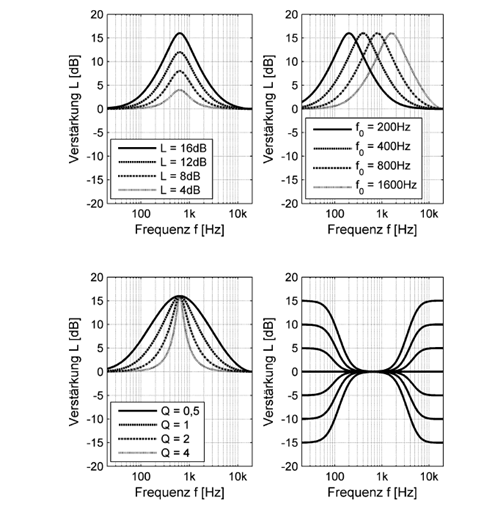
\includegraphics[scale=.5]{graph/filter}}
			\end{figure}
		}
		\only<2>{
			\begin{itemize}
				\item	\textbf{low pass \& high pass}
					\begin{itemize}
						\item	cut-off frequency, slope, (resonance)
					\end{itemize}
				\item	\textbf{low shelving \& high shelving}
					\begin{itemize}
						\item	cut-off frequency, gain
					\end{itemize}
				\item	\textbf{peak filter}
					\begin{itemize}
						\item	mid frequency, gain, bandwidth/Q
					\end{itemize}
				\item	\textbf{band pass \& bad elimination}
					\begin{itemize}
						\item	mid frequency, bandwidth/Q, slope
					\end{itemize}
				\item	\textbf{notch}
					\begin{itemize}
						\item	(mid) frequency
					\end{itemize}
			\end{itemize}
		}
	\end{frame}
	\begin{frame}{filter}{traditional filter applications}
		\begin{itemize}
			\item	audio equalizing
			\pause
			\item	removal of unnecessary/unwanted components: DC, Hum
			\pause
			\item	emphasis/de-emphasis
			\pause
			\item	(parameter) smoothing
				\begin{figure}
					\centerline{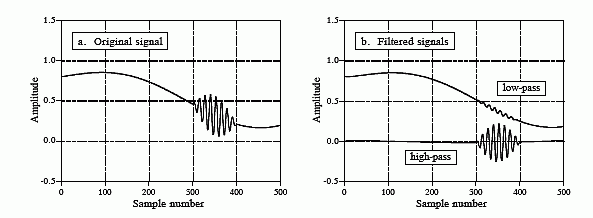
\includegraphics[scale=.6]{graph/parameter_smoothing}}
				    \label{fig:parameter_smoothing}
				\end{figure}
		\end{itemize}
	\end{frame}
	
	\begin{frame}{filter}{digital filter description}
		filter is completely defined by its
		\begin{itemize}
			\item	complex transfer function $H(\mathrm{j}\omega)$, or its
			\item	impulse response $h(t)$, or its
			\item	list of pole and zero positions in the Z-plane
		\end{itemize}
		\pause
		\begin{equation}
			H(\mathrm{j}\omega) = \mathfrak{F}\{h(t)\}
		\end{equation}
	\end{frame}


	
	\begin{frame}{filter}{example 1}
	        \begin{figure}
				\begin{center}
	            \begin{picture}(50,30)
	
	                %boxes
	                \put(25,5){\framebox(7,6){\footnotesize{$z^{-1}$}}}
	
	                %lines horizontal
	                \put(5,20){\vector(1,0){22.5}}
	                \put(29.5,20){\vector(1,0){11.5}}
	                \put(43,20){\vector(1,0){10}}
	                
	                \put(15,8){\vector(1,0){10}}
	                \put(32,8){\line(1,0){10}}
	
	                %lines vertical
	                \put(15,20){\line(0,-1){12}}
	                \put(42,8){\vector(0,1){4}}
	                \put(42,14){\vector(0,1){5}}
	                
	                %circles
	                \put(27,19){$\otimes$}
	                \put(40.5,19){$\oplus$} % 42-20
	                \put(40.5,12){$\otimes$}
	                
	                \put(15,20){\circle*{1}}
	
	                %text
	                \put(26,24){\footnotesize{\shortstack[c]{$\nicefrac{1}{2}$}}}
	                \put(46,10){\footnotesize{\shortstack[c]{$\nicefrac{1}{2}$}}}
	
	                \put(4,22){\footnotesize{\shortstack[c]{x(n)}}}
	                \put(52,22){\footnotesize{\shortstack[c]{y(n)}}}
	
	            \end{picture}
				\end{center}
	        \end{figure}
        
        	\begin{equation}
        		y(n) = 0.5\cdot x(n) + 0.5\cdot x(n-1)
        	\end{equation}
	\end{frame}	
	
	\begin{frame}{filter}{example 1: transfer function 1/2}
    	\begin{eqnarray}
	        		y(n) &=& 0.5\cdot x(n) + 0.5\cdot x(n-1)\\
	        		H(z) &=& 0.5  + 0.5\cdot z^{-1}\\
	       	\pause
	        		H(j\omega) &=& 0.5  + 0.5\cdot e^{-j\omega}\\
	       	\pause
	       			|H(j\omega)| &=&0.5 \cdot \left| e^{-j\frac{\omega}{2}} \cdot \left( e^{j\frac{\omega}{2}} + e^{-j\frac{\omega}{2}}\right)\right| \\
	       	\pause
	       				&=&0.5 \cdot \underbrace{\left| e^{-j\frac{\omega}{2}}\right|}_{1} \cdot  \underbrace{\left|\left( e^{j\frac{\omega}{2}} + e^{-j\frac{\omega}{2}}\right)\right|}_{\left| 2\cos\left(\frac{\omega}{2}\right) \right|} \\
	       	\pause
	       	&=& \left| \cos\left(\frac{\omega}{2}\right) \right|
    	\end{eqnarray}
	\end{frame}	
	
	\begin{frame}{filter}{example 1: transfer function 2/2}
		\begin{figure}
			\centerline{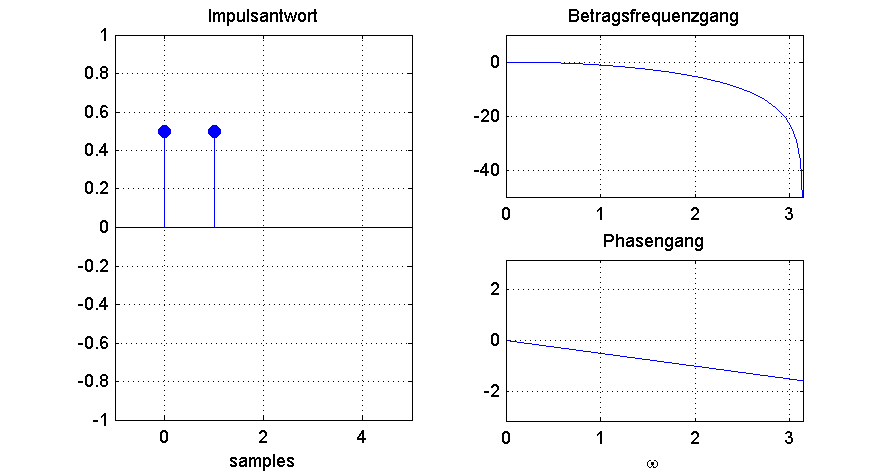
\includegraphics[scale=.5]{graph/fx_01}}
		    \label{fig:fx_01}
		\end{figure}
	\end{frame}	
	
	\begin{frame}{filter}{example 2}
        \begin{figure}
			\begin{center}
            \begin{picture}(50,30)

                %boxes
                \put(25,5){\framebox(7,6){\footnotesize{$z^{-1}$}}}

                %lines horizontal
                \put(5,20){\vector(1,0){22.5}}
                \put(29.5,20){\vector(1,0){11.5}}
                \put(43,20){\vector(1,0){10}}
                
                \put(15,8){\vector(1,0){10}}
                \put(32,8){\line(1,0){10}}

                %lines vertical
                \put(15,20){\line(0,-1){12}}
                \put(42,8){\vector(0,1){4}}
                \put(42,14){\vector(0,1){5}}
                
                %circles
                \put(27,19){$\otimes$}
                \put(40.5,19){$\oplus$} % 42-20
                \put(40.5,12){$\otimes$}
                
                \put(15,20){\circle*{1}}

                %text
                \put(26,24){\footnotesize{\shortstack[c]{$\nicefrac{1}{2}$}}}
                \put(46,10){\footnotesize{\shortstack[c]{$-\nicefrac{1}{2}$}}}

                \put(4,22){\footnotesize{\shortstack[c]{x(n)}}}
                \put(52,22){\footnotesize{\shortstack[c]{y(n)}}}

            \end{picture}
			\end{center}
        \end{figure}
        \pause
    	\begin{eqnarray}
    		y(n) &=& 0.5\cdot x(n) - 0.5\cdot x(n-1)\\
    		H(z) &=& 0.5  - 0.5\cdot z^{-1}\\
    	\pause
    		|H(j\omega)| &=& \left| \sin\left(\frac{\omega}{2}\right) \right|
    	\end{eqnarray}
	\end{frame}	
	
	\begin{frame}{filter}{example 2: transfer function}
		\begin{figure}
			\centerline{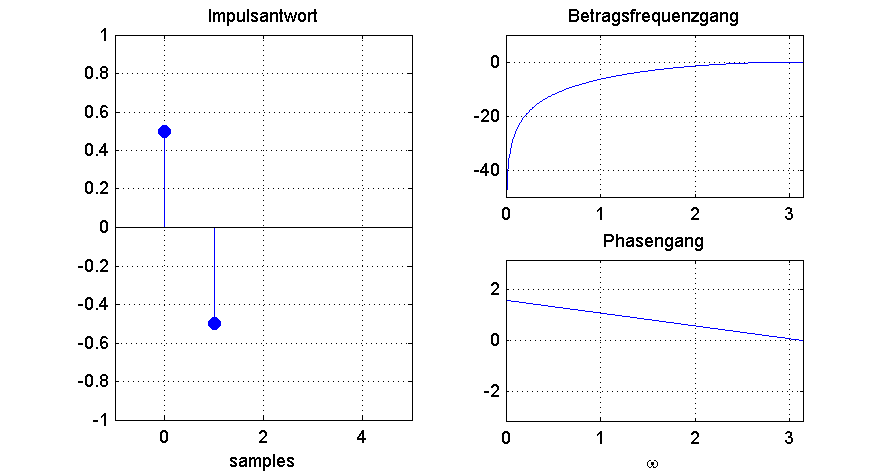
\includegraphics[scale=.5]{graph/fx_02}}
		\end{figure}
	\end{frame}	
	
	\begin{frame}{filter}{example 3}
       \begin{figure}[!hbt]
			\begin{center}
            \begin{picture}(50,30)

                %boxes
                \put(25,5){\framebox(7,6){\footnotesize{$z^{-N}$}}}

                %lines horizontal
                \put(5,20){\vector(1,0){22.5}}
                \put(29.5,20){\vector(1,0){11.5}}
                \put(43,20){\vector(1,0){10}}
                
                \put(15,8){\vector(1,0){10}}
                \put(32,8){\line(1,0){10}}

                %lines vertical
                \put(15,20){\line(0,-1){12}}
                \put(42,8){\vector(0,1){4}}
                \put(42,14){\vector(0,1){5}}
                
                %circles
                \put(27,19){$\otimes$}
                \put(40.5,19){$\oplus$} % 42-20
                \put(40.5,12){$\otimes$}
                
                \put(15,20){\circle*{1}}

                %text
                \put(26,24){\footnotesize{\shortstack[c]{$\nicefrac{1}{2}$}}}
                \put(46,10){\footnotesize{\shortstack[c]{$-\nicefrac{1}{2}$}}}

                \put(4,22){\footnotesize{\shortstack[c]{x(n)}}}
                \put(52,22){\footnotesize{\shortstack[c]{y(n)}}}

            \end{picture}
			\end{center}
        \end{figure}
		\pause      
    	\begin{eqnarray}
    		y(n) &=& 0.5\cdot x(n) - 0.5\cdot x(n-N)\\
    		H(z) &=& 0.5  - 0.5\cdot z^{-N}\\
			\pause
    		|H(j\omega)| &=& 0.5\cdot\left| e^{-j\frac{N\omega}{2}} \cdot \left(e^{j\frac{N\omega}{2}} - e^{-j\frac{N\omega}{2}} \right) \right|\\
			\pause
    		 &=& \left| \sin\left(\frac{N\omega}{2}\right) \right|
    	\end{eqnarray}
	\end{frame}	
	
	\begin{frame}{filter}{example 3: transfer function}
		\begin{figure}
			\centerline{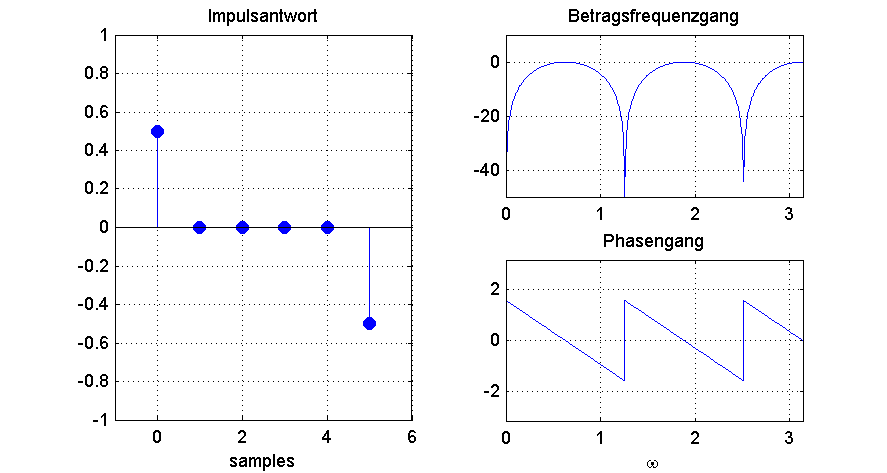
\includegraphics[scale=.5]{graph/fx_03}}
		    \label{fig:fx_03}
		\end{figure}
	\end{frame}	
	
	\begin{frame}{filter}{example 4}
        \begin{figure}
			\begin{center}
            \begin{picture}(50,70)

                %boxes
                \put(25,50){\framebox(7,6){\footnotesize{$z^{-1}$}}}
                \put(25,38){\framebox(7,6){\footnotesize{$z^{-2}$}}}
                \put(28,28){\shortstack[c]{$\vdots$}}
                \put(21,14){\framebox(14,6){\footnotesize{$z^{-(\mathcal{J}-1)}$}}}

                %lines horizontal
                \put(5,65){\vector(1,0){22.5}}
                \put(29.5,65){\vector(1,0){11.5}}
                \put(43,65){\vector(1,0){10}}
                
                \put(15,53){\vector(1,0){10}}
                \put(32,53){\vector(1,0){4}}
                \put(38,53){\vector(1,0){3}}
                
                \put(15,41){\vector(1,0){10}}
                \put(32,41){\vector(1,0){4}}
                \put(38,41){\vector(1,0){3}}
                
                \put(15,29){\vector(1,0){10}}
                \put(32,29){\vector(1,0){4}}
                \put(38,29){\vector(1,0){3}}
                
                \put(15,17){\vector(1,0){6}}
                \put(35,17){\line(1,0){7}}

                %lines vertical
                \put(15,65){\line(0,-1){48}}
                \put(42,54){\vector(0,1){10}}
                %\put(42,60){\vector(0,1){4}}
                
                \put(42,42){\vector(0,1){10}}
                %\put(42,48){\vector(0,1){4}}
                
                \put(42,30){\vector(0,1){10}}
                %\put(42,36){\vector(0,1){4}}
                
                \put(42,17){\vector(0,1){5}}
                \put(42,24){\vector(0,1){4}}
                
                %circles
                \put(27,64){$\otimes$}
                \put(40.5,64){$\oplus$} % 42-20
                \put(40.5,52){$\oplus$} % 42-20
                \put(40.5,40){$\oplus$} % 42-20
                \put(40.5,28){$\oplus$} % 42-20
                
                \put(35.5,52){$\otimes$}
                \put(35.5,40){$\otimes$}
                \put(35.5,28){$\otimes$}
                \put(40.5,22){$\otimes$}
                
                \put(15,65){\circle*{1}}
                \put(15,53){\circle*{1}}
                \put(15,41){\circle*{1}}
                \put(15,29){\circle*{1}}

                %text
                \put(26,69){\footnotesize{\shortstack[c]{$\nicefrac{1}{\mathcal{J}}$}}}
                \put(35,57){\footnotesize{\shortstack[c]{$\nicefrac{1}{\mathcal{J}}$}}}
                \put(35,45){\footnotesize{\shortstack[c]{$\nicefrac{1}{\mathcal{J}}$}}}
                \put(35,33){\footnotesize{\shortstack[c]{$\nicefrac{1}{\mathcal{J}}$}}}
                \put(44,21){\footnotesize{\shortstack[c]{$\nicefrac{1}{\mathcal{J}}$}}}

                \put(4,67){\footnotesize{\shortstack[c]{x(n)}}}
                \put(52,67){\footnotesize{\shortstack[c]{y(n)}}}

            \end{picture}
			\end{center}
        \end{figure}
        
    	\vspace{-20mm}
    	\begin{equation}
    		y(n) = \frac{1}{\mathcal{J}}\sum_{j=0}^{\mathcal{J}-1} x(n-j)
    	\end{equation}
	\end{frame}
	\begin{frame}{filter}{example 4: transfer function}
		\begin{figure}
			\centerline{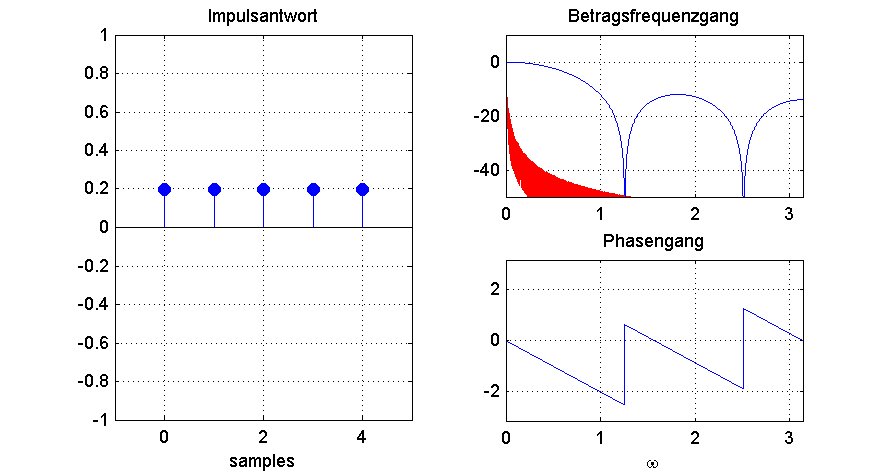
\includegraphics[scale=.5]{graph/fx_04}}
		\end{figure}
    	\begin{equation}
    		H(j\omega) = e^{-\mathrm{j}\mathcal{J}\frac{\omega}{2}}\frac{\sin\left(\mathcal{J}\cdot\frac{\omega}{2} \right)}{\mathcal{J}\cdot\sin\left(\frac{\omega}{2} \right)}
    	\end{equation}
	\end{frame}	
	\begin{frame}{filter}{example 4: recursive implementation}
		\begin{eqnarray}
			y(i) &=& \sum\limits_{j=0}^{\mathcal{J}-1}{\frac{1}{\mathcal{J}}\cdot x(i-j)}\nonumber\\
			\pause
			&=& \frac{1}{\mathcal{J}}\cdot \big(x(i) - x(i-\mathcal{J})\big) + \underbrace{\sum\limits_{j=1}^{\mathcal{J}}{\frac{1}{\mathcal{J}}\cdot x(i-j)}}_{y(i-1)}\nonumber\\
			\pause
			&=& \frac{1}{\mathcal{J}}\cdot \big(x(i) - x(i-\mathcal{J})\big) + y(i-1) 
		\end{eqnarray} 
		\pause
		\textcolor{blue}{not applicable with windowed coefficients!}
	\end{frame}
	\begin{frame}{filter}{example 5}
	        \begin{figure}[!hbt]
				\begin{center}
	            \begin{picture}(50,30)
	
	                %boxes
	                \put(25,5){\framebox(7,6){\footnotesize{$z^{-1}$}}}
	
	                %lines horizontal
	                \put(0,20){\vector(1,0){6}}
	                \put(8,20){\vector(1,0){47}}
	                
	                \put(15,8){\line(1,0){10}}
	                \put(42,8){\vector(-1,0){10}}
	
	                %lines vertical
	                \put(42,20){\line(0,-1){12}}
	                \put(15,8){\vector(0,1){4}}
	                \put(15,14){\vector(0,1){5}}
	                
	                %circles
	                \put(5.5,19){$\otimes$}
	                \put(13.5,19){$\oplus$} % 15-20
	                \put(13.5,12){$\otimes$}
	                
	                \put(42,20){\circle*{1}}
	
	                %text
	                \put(4,22){\footnotesize{\shortstack[c]{$(1-\alpha)$}}}
	                \put(11,10){\footnotesize{\shortstack[c]{$\alpha$}}}
	
	                \put(-2,22){\footnotesize{\shortstack[c]{x(n)}}}
	                \put(52,22){\footnotesize{\shortstack[c]{y(n)}}}
	
	            \end{picture}
				\end{center}
	        \end{figure}
        	\begin{eqnarray}
        		y(n) &=& (1-\alpha)\cdot x(n) + \alpha\cdot y(n-1)\\
        			&=& x(n) + \alpha \cdot (y(n-1) - x(n))
        	\end{eqnarray}
	\end{frame}
	
	\begin{frame}{Example 5: transfer function 1/2}
    	\begin{eqnarray}
        		y(n) &=& (1-\alpha)\cdot x(n) + \alpha\cdot y(n-1)\\
        		H(z) &=& \frac{1-\alpha}{1-\alpha z^{-1}}\\
        \pause
        		H(j\omega) &=& \frac{1-\alpha}{1-\alpha e^{-j\omega}}\\
        \pause
        		|H(j\omega)| &=& \left|\frac{1-\alpha}{1-\alpha e^{-j\omega}}\right| \\
        \pause
        		&=&\frac{1-\alpha}{\sqrt{(1 + \alpha^2 - 2\alpha\cos(\omega)}} 
    	\end{eqnarray}
	\end{frame}
	\begin{frame}{filter}{example 5: transfer function 2/2}
		\begin{figure}
			\centerline{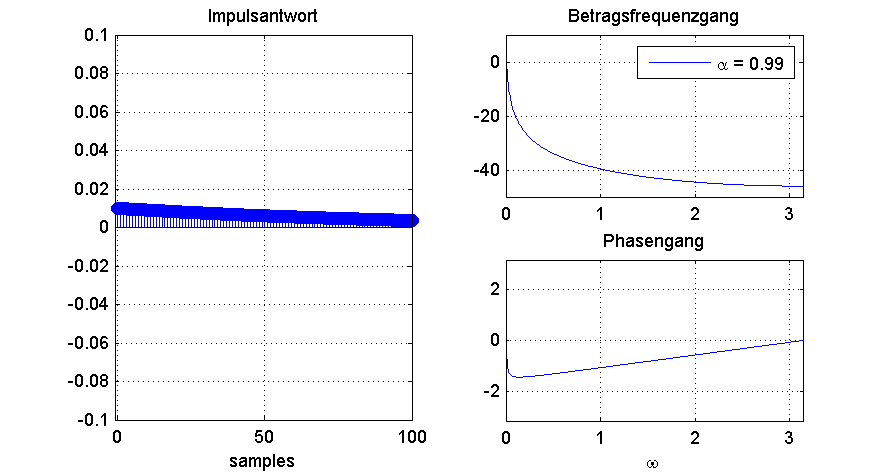
\includegraphics[scale=.5]{graph/fx_05}}
		\end{figure}
	\end{frame}
	\begin{frame}{filter}{example 6}
        \begin{figure}[!hbt]
			\begin{center}
            \begin{picture}(50,30)

                %boxes
                \put(25,5){\framebox(7,6){\footnotesize{$z^{-N}$}}}

                %lines horizontal
                \put(0,20){\vector(1,0){14}}
                \put(16,20){\vector(1,0){32}}
                \put(50,20){\vector(1,0){5}}
                
                \put(15,8){\line(1,0){10}}
                \put(42,8){\vector(-1,0){10}}

                %lines vertical
                \put(42,20){\line(0,-1){12}}
                \put(15,8){\vector(0,1){4}}
                \put(15,14){\vector(0,1){5}}
                
                %circles
                \put(47.5,19){$\otimes$}
                \put(13.5,19){$\oplus$} % 15-20
                \put(13.5,12){$\otimes$}
                
                \put(42,20){\circle*{1}}

                %text
                \put(43,22){\footnotesize{\shortstack[c]{$b_0$}}}
                \put(8,10){\footnotesize{\shortstack[c]{$-a_N$}}}

                \put(-2,22){\footnotesize{\shortstack[c]{x(n)}}}
                \put(52,22){\footnotesize{\shortstack[c]{y(n)}}}

            \end{picture}
			\end{center}
        \end{figure}
    	\begin{equation}
    		y(n) = b_0\cdot x(n) - a_N\cdot y(n-N)
    	\end{equation}
	\end{frame}
	\begin{frame}{filter}{example 6: transfer function}
		\begin{figure}
			\centerline{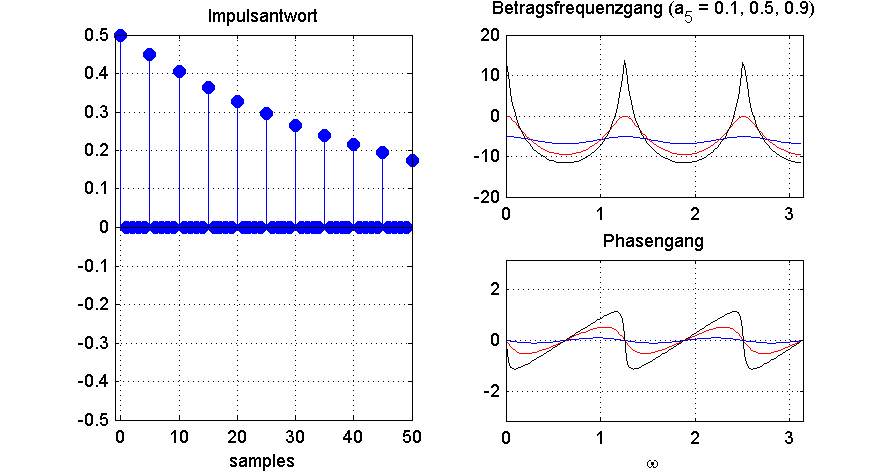
\includegraphics[scale=.5]{graph/fx_06}}
		    \label{fig:fx_06}
		\end{figure}
    	\begin{equation}
    		H(j\omega) = \frac{b_0}{1-a_N\cdot e^{-j\omega N}}
    	\end{equation}
	\end{frame}
	\begin{frame}{filter}{biquad: structure}
		\begin{figure}
			\centerline{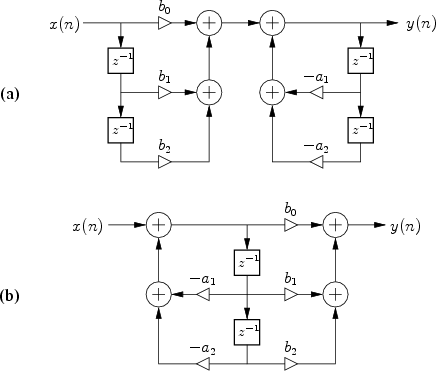
\includegraphics[scale=.3]{graph/general_biquad_jos}}
		    \label{fig:general_biquad}
		\end{figure}
		\pause
		\vspace{-3mm}
		\begin{eqnarray}
			\text{diff eq}: y(n) 	&=& \sum_{k=0}^{K_1}{b_k\cdot x(n-k)} + \sum_{k=1}^{K_2}{-a_k\cdot y(n-k)} \nonumber\\
			\text{trans. fct}: H(z) 	&=& \frac{Y(z)}{X(z)} =  \frac{\sum_{k=0}^{K_1}{b_k\cdot z^{-k}}}{1 + \sum_{k=1}^{K_2}{a_k\cdot z^{-k}}} 
		\end{eqnarray}
	\end{frame}
	
	\begin{frame}\frametitle{filter}\framesubtitle{z-plane}
			\begin{figure}[!hbt]
				\begin{center}
					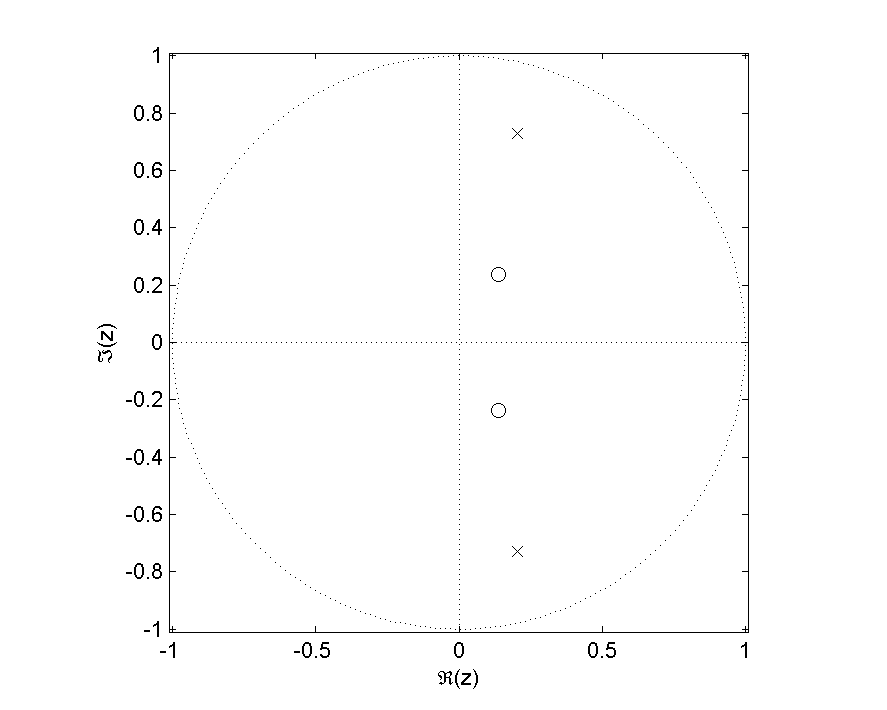
\includegraphics[scale=.6]{graph/PoleZero}
				\end{center}
			\end{figure}
	\end{frame}
	
	\begin{frame}\frametitle{filter}\framesubtitle{z-plane: animation}
		%\begin{figure}
			%\includemovie[poster,mouse=true]{\linewidth}{.7\linewidth}{video/PoleZero.avi}
		%\end{figure}
	\end{frame}
	
	\begin{frame}\frametitle{filter}\framesubtitle{z-plane: 3D-view}
			\begin{figure}[!hbt]
				\begin{center}
					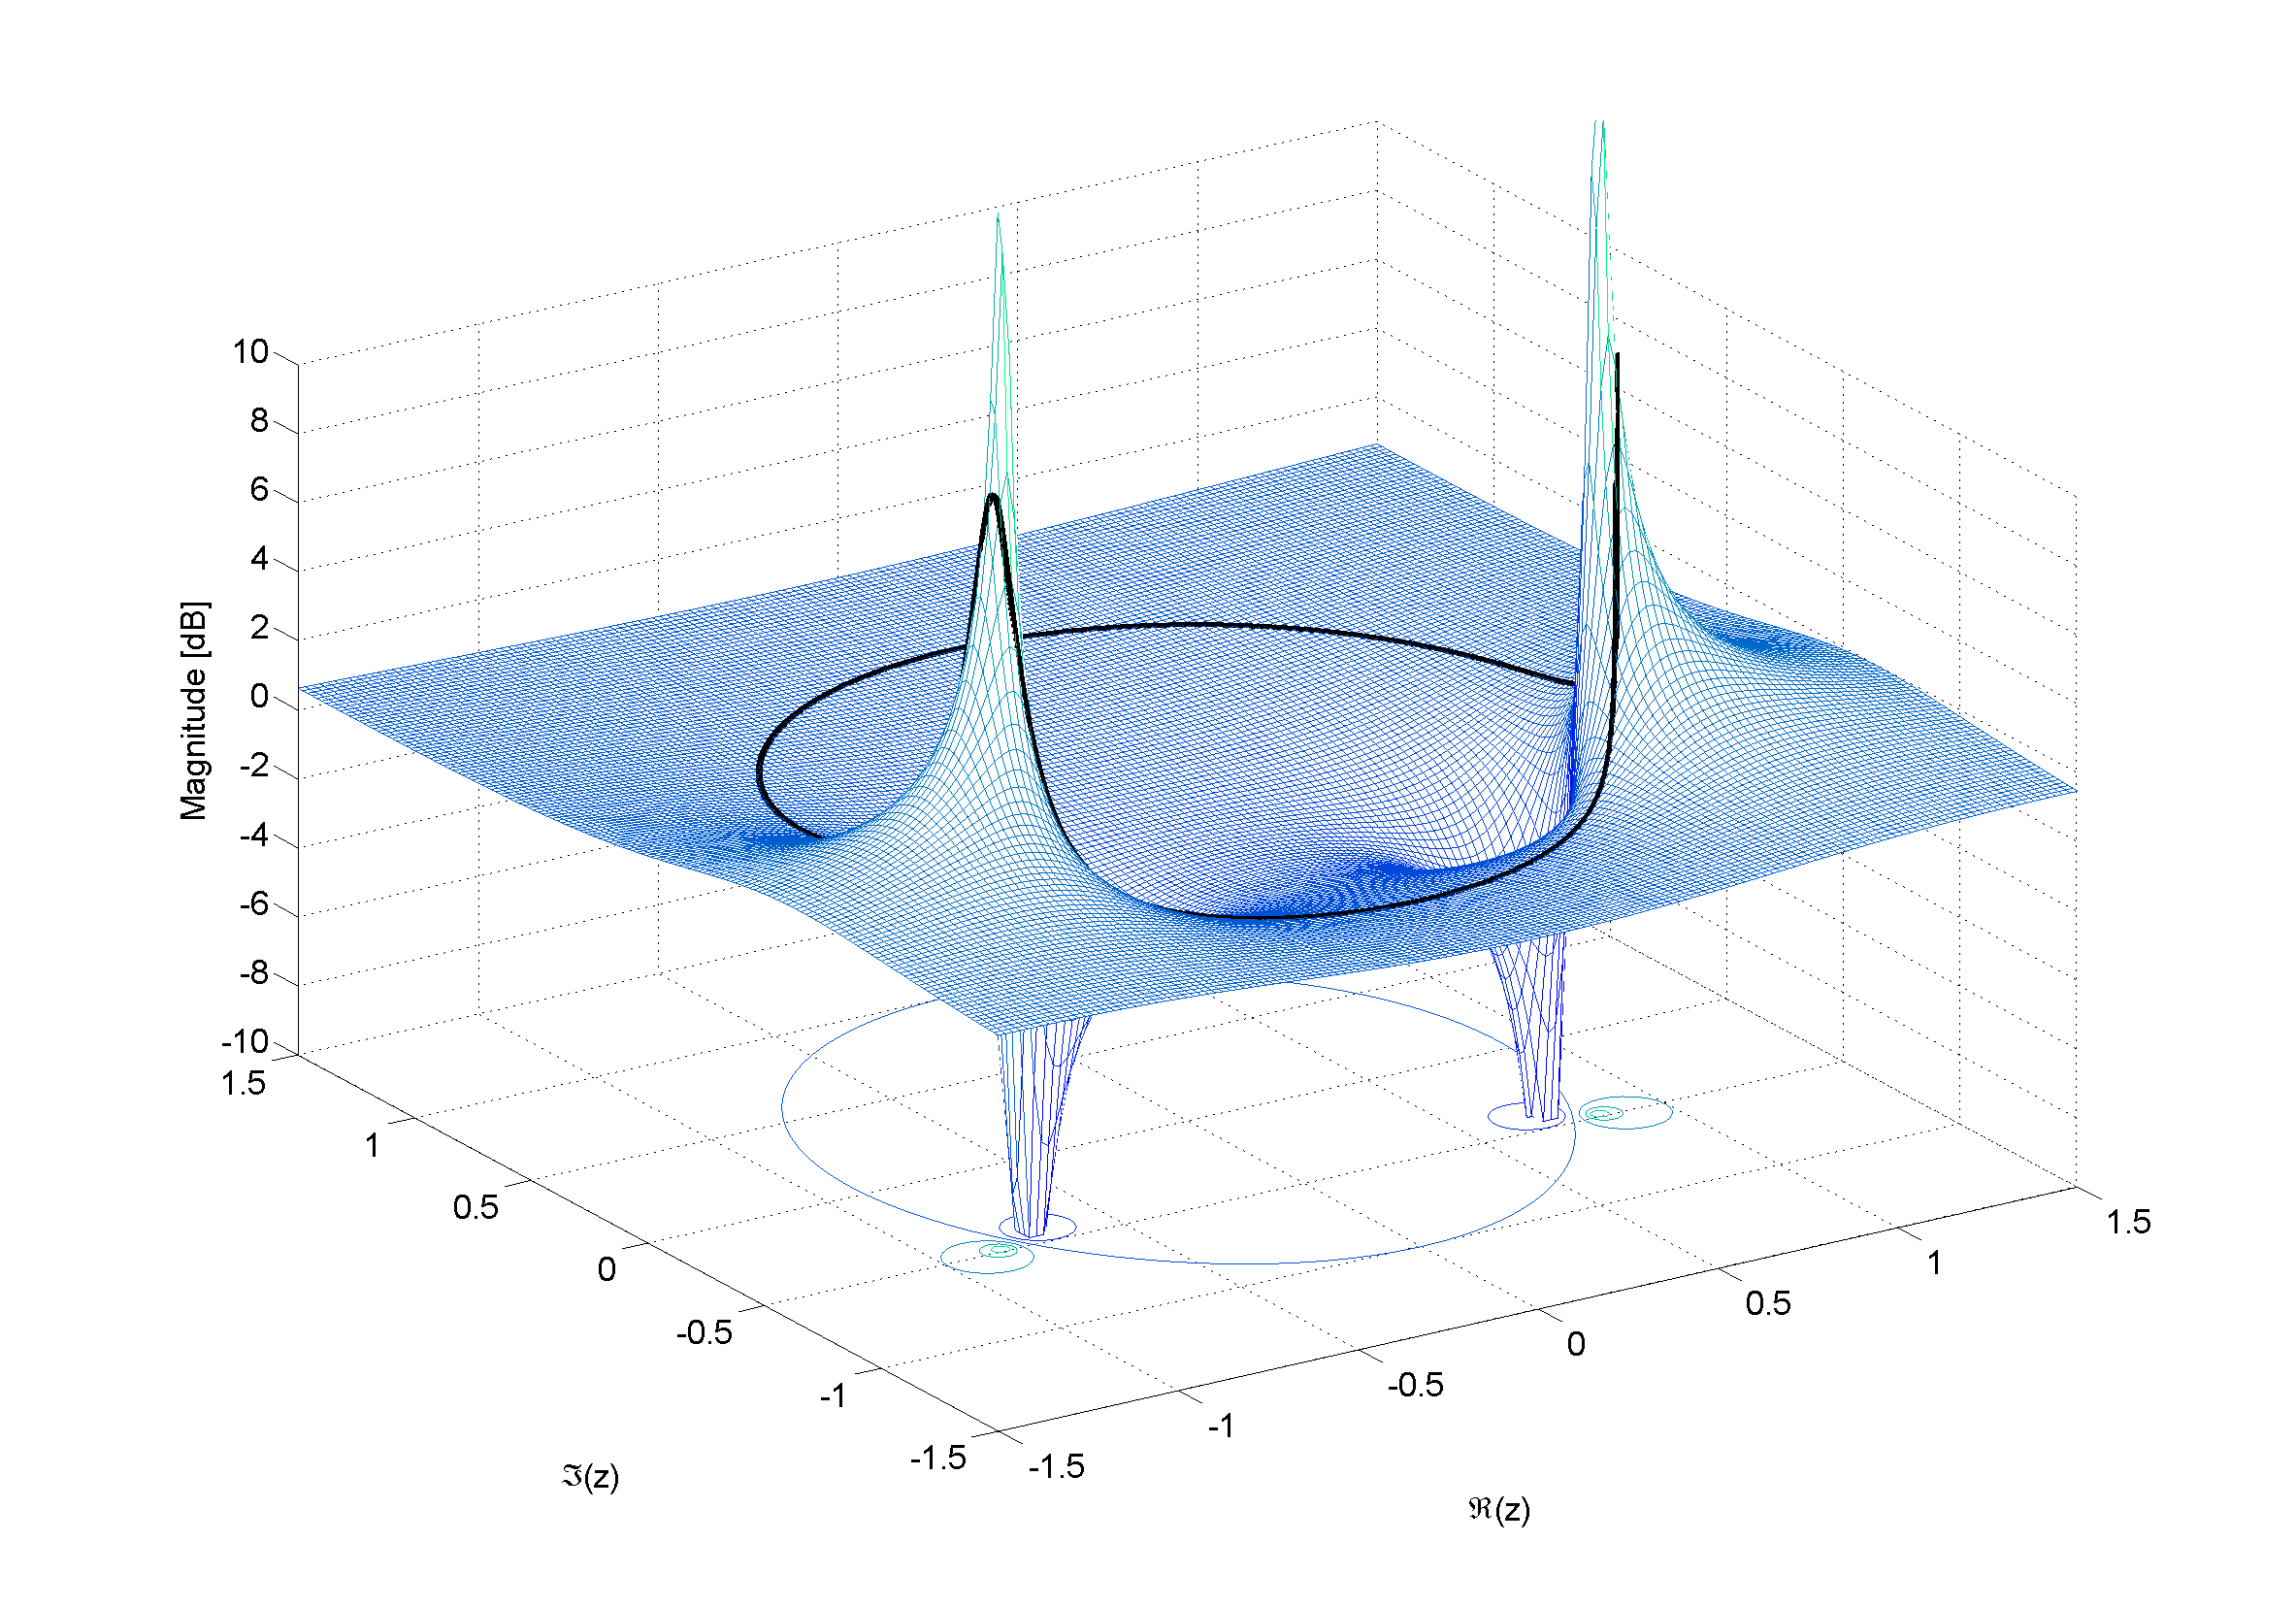
\includegraphics[scale=.26]{graph/PoleZero3d}
				\end{center}
			\end{figure}
	\end{frame}
	
	\begin{frame}{filter}{filter design}
		\begin{itemize}
			\item	\textbf{FIR}: coefficients are measured impulse response
			\pause
			\item	\textbf{bilinear transform}: analogue prototype
			\pause
			\item	\textbf{z-plane}: move poles and zeros
			\item	\ldots	
		\end{itemize}
	\end{frame}
	
	\begin{frame}{filter}{FIR \& IIR}
		\begin{itemize}
			\item	impulse response length (finite vs.\ infinite)
			\pause
			\item	structure (no feedback vs.\ feedback)
			\pause
			\item	phase linearity (possible vs.\ impossible)
					\pause
					
					FIR with linear phase (constant group delay) if
					\begin{eqnarray}
						h(n) =& h(N-n) & 0\leq n\leq N\\
						h(n) =& -h(N-n) & 0\leq n\leq N
					\end{eqnarray}
			\pause
			\item	ratio steepness to workload (high vs. low)
			\pause
			\item	stability (perfect vs.\ possibly instable)
		\end{itemize}
	\end{frame}

		\begin{frame}{filter}{zero-phase filtering with IIR 1/2}
			Apply filter wird forwards and backwards ($\rightarrow$ symmetric IR)
			\begin{eqnarray}
				y_{tmp}(n) &=& h(n)*x(n)\\
				y (n) &=& flip(h(n)*flip(y_{tmp}(n)))
			\end{eqnarray}
				\begin{figure}
					\centerline{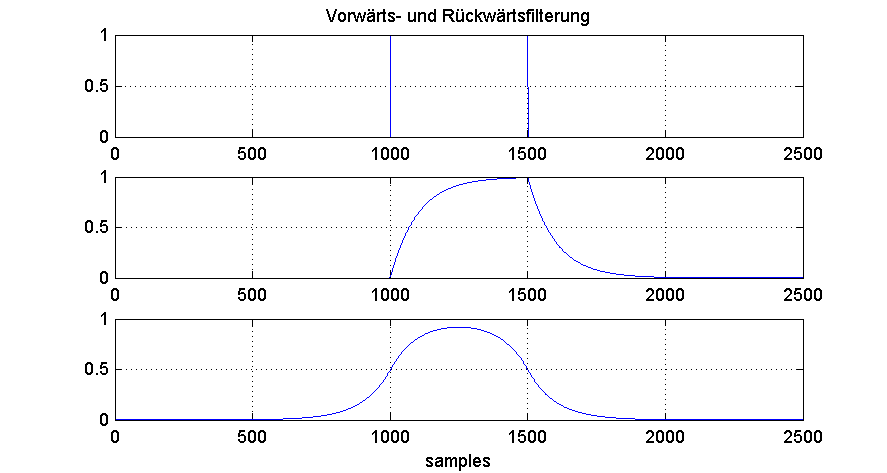
\includegraphics[scale=.5]{graph/fx_07}}
				    \label{fig:fx_07}
				\end{figure}
		\end{frame}
		\begin{frame}{filter}{zero-phase filtering with IIR 2/2}
			Derivation
			\begin{eqnarray}
				y (n) &=& flip(h(n)*flip(y_{tmp}(n)))\\
					&=& flip(h(n))*y_{tmp}(n)\\
					&=& flip(h(n))*(h(n)*x(n))
			\end{eqnarray}
			\begin{equation}
				\mathcal{Z}\{flip(h(n))\} = H(z^{-1})
			\end{equation}
			\begin{eqnarray}
				Y(z) &=& H(z^{-1})*\left(H(z)\cdot X(z)\right)\\
				Y(j\omega)	&=& H(-j\omega) \cdot H(j\omega) \cdot X(j\omega)\\
					&=& |H(j\omega)|^2\cdot X(j\omega)
			\end{eqnarray}
		\end{frame}
	
	\begin{frame}{filter}{FIR: FFT filtering}
			\begin{eqnarray}
				x(n)\ast h(n) &=& \mathfrak{F}^{-1}\{X(j\omega)\cdot H(j\omega)\}\\
								&=&\mathfrak{F}^{-1}\{\mathfrak{F}{x}\cdot \mathfrak{F}{h}\}
			\end{eqnarray}
			efficient computation for long FIR filters
			
			\pause
			BUT:
			\begin{itemize}
				\item	only for \textit{complete} signal $\rightarrow$ latency
				\item	FFT length has to be
					\begin{itemize}
						\item	power of 2
						\item	identical for both IR and signal
						\item	$\geq$ L(x) + L(h) 
					\end{itemize}
			\end{itemize}
	\end{frame}
	\begin{frame}{filter}{all-pass filter}
   \begin{figure}[!hbt]
		\begin{center}
        \begin{picture}(30,40)

            %boxes
            \put(11,21){\framebox(8,8){\footnotesize{$z^{-M}$}}}

		
            %lines horizontal
            \put(0,25){\vector(1,0){11}}
            \put(19,25){\vector(1,0){10}}

            \put(31,25){\vector(1,0){4}}
            \put(5,35){\vector(1,0){9}}
            \put(16,35){\line(1,0){14}}
            
            \put(0,15){\line(1,0){14}}
            \put(25,15){\vector(-1,0){9}}
            \put(-5,25){\vector(1,0){4}}
            
            %lines vertical
            \put(5,25){\line(0,1){10}}
            \put(30,35){\line(0,-1){9}}
            
            \put(0,15){\vector(0,1){9}}
            \put(25,25){\line(0,-1){10}}
            
            %circles
            \put(13.5,34){$\otimes$} %15,35
            \put(28.5,24){$\oplus$} % 30,25
            \put(13.5,14){$\otimes$} % 
            \put(-1.5,24){$\oplus$} % 0,25
            
            \put(5,25){\circle*{1}}
            \put(25,25){\circle*{1}}

            %text
            \put(-5,28){\footnotesize{\shortstack[c]{x(n)}}}
            \put(35,28){\footnotesize{\shortstack[c]{y(n)}}}
            \put(16,36){\footnotesize{\shortstack[c]{-g}}}
            \put(16,12){\footnotesize{\shortstack[c]{g}}}

        \end{picture}
		\end{center}
    \end{figure}
	\begin{eqnarray}
		y(n) &=& g\cdot x(n) + x(n-M) - g\cdot y(n-M)\\
		H(z) &=& \frac{z^{-M} - g}{1 - g\cdot z^{-M}}
	\end{eqnarray}
	\end{frame}
